\section{Ecosystem Simulator} \label{sec:ecosystem_simulator}

Once the user selects the union of all species to appear in all clusters of the terrain, it is necessary to determine a valid vegetation distribution for each. To do so, an ecosystem simulator is used as in the work of Deussen et al \cite{Deussen1998} and Lane and Przemyslaw \cite{Lane2002}. Unlike these other ecosystem simulators, however, our approach is not based on L-Systems, and models both resource requirements and resource availability in greater detail. The purpose of the ecosystem simulator is to determine, given a vegetation state, \textit{S$_{t}$} at time \textit{t}, the state \textit{S$_{t+n}$} at time \textit{t+n}, for any value of n. To do so, the simulation advances through time at monthly intervals and the strength of all plant instances are iteratively re-calculated. This strength of a given plant depends on it's age, available resources and surrounding plants with which it is competing for resources. This calculated value directly influences the plants growth and ability to survive.\\

\subsection{Gridded Simulation Area}

The simulation area greatly effects the performance of the ecosystem simulator and, therefore, it is necessary to keep it to a minimum. However, too small a simulation area will fail to accurately model the interaction of larger plant species. Given these constraints, a simulation window of one hundred by one hundred meters is used, accurate to the nearest centimetre. This area is deemed conservative, however, as rare are the species which come remotely close to such spatial coverage. An extension to this work would be to adjust the size of the simulation window depending on the  species selected. This would ensure optimal simulation speed for all simulation runs. \\

When iteratively calculating the strength of plant instances, it is necessary to quickly determine the set of plants S = \{P$_{1}$, P$_{2}$, P$_{3}$, ...\} competing for available resources with \textit{P$_{n}$}. Determining \textit{S} depends on the spatial reach of \textit{P$_{n}$}. Spatial awareness is therefore a key requirement of the simulation and is achieved by splitting the simulation window into a grid of smaller cells. \\

The size of individual cells can be configured to increase or decrease the resolution and, therefore, the accuracy of the simulation. As the simulation progresses, plants grow, their spatial coverage increases, and they enter new grid cells. When a plant enters a new grid cell, it becomes a member and cell resources are distributed to it. The information associated with each individual grid cell can be split into two categories: \textit{time-dependent} and \textit{simulation-dependent}. The time-dependent information depends only on the current month, is identical for every grid cell and comprised of: the \textit{soil moisture} and the \textit{illumination}. The simulation-dependent information varies throughout the simulation as plants spawn, die and grow and consists of: the \textit{list of plants whose roots intersect the cell} and the \textit{list of plants whose canopy intersects the cell}. It is important to have both as plant roots and canopies grow at different rates and their cell coverage will therefore differ. \\
By employing this gridded approach, determining the set of plants which compete for resources is extremely efficient. For example, to determine the set of plants with which \textit{P$_{n}$} is competing for soil moisture, it is only necessary to determine the cells covered by its roots, which depends solely on its position and root size.\\
Another advantage of this gridded approach, which is discussed in further detail below, is that it splits plants into separate cells, each with unique resource distributions. This permits partial shading, for example, where illumination is zero in some of its cells but more in others. \\

\subsection{Soil Moisture Distribution} \label{subsec:humidity_distribution}

Plants grow their roots in order to access the nutrients and moisture available in the surrounding soil. As roots of different plant instances overlap, they compete for these resources. A notable simplification in our work is that soil depth is not modelled. Soil depth affects the plants rooting reach and has a significant impact on plant growth \cite{Fourcaud2008}. A a future extension to this work, the soil could be modelled as layers, which would permit plants to battle for different soil resources depending on their root depth. For example, grass and shrub with small root depth would access soil moisture in the upper most layer but large trees would access it in the deeper most layer. They would therefore not be competing for soil moisture. \\

The strength of each plant in the simulation must be recalculated on a monthly basis. Part of the information required to calculate the overall strength of a given plant is the moisture allocated to it, which is taken as the average of the moisture allocated to it in each cell its roots overlap. To determine the overall moisture allocated to a given plant \textit{p}, it is first necessary, therefore, to iterate over all incident grid cells and calculate the moisture allocated to each plant with intersecting roots.\\

When distributing the soil moisture in a given grid cell \textit{C$_{xy}$} to the set \textit{S} = \{P$_{1}$, P$_{2}$, P$_{3}$, ...\} of plants whose roots intersect the cell, one of three distinct scenarios can occur, depending on the available moisture, \textit{M$_{available}$}, of the cell: \textit{Abundant}, \textit{sufficient} and \textit{insufficient}.\\

The moisture is deemed abundant if the available moisture, \textit{M$_{available}$}, surpasses 300 millimetres. To prevent situations where the soil moisture attributed to a given plant is small simply because the majority of the available moisture is distributed to other plants, all plants of \textit{S} are allocated \textit{M$_{available}$}. This is important as it could lead to situations where species strive in areas completely unsuited. The available soil moisture is directly dependent on rainfall. At three hundred millimetres, rainfall can be considered abundant and soil moisture therefore not a limiting factor. \\

If \textit{M$_{available}$} is less than 300 millimetres, it is necessary to determine whether the moisture is sufficient or insufficient by calculating the requested moisture \textit{M$_{requested}$}, as outlined in equation \ref{eq:humidity_requested_calc}. \\

\begin{equation}
M_{requested} = \sum MinMoisture(P_{n}) \text{ for } n \in S
\label{eq:humidity_requested_calc}
\end{equation}
Where: \textit{MinMoisture(P$_{n}$)} is the minimum moisture requirement of the species to which plant \textit{P$_{n}$} belongs; \textit{S} is the set of plants whose roots intersect the given grid cell.\\

If \textit{M$_{requested}$} is less than \textit{M$_{available}$}, the moisture is deemed sufficient and the amount allocated to each plant is calculated as described in equation \ref{eq:humidity_allocation_sufficient_calc}. Intuitively, this equation allocates each plant with the minimum amount of humidity it requires to survive plus the resulting overflow. Note that in this equation, the overflow is not distributed amongst plants of the cell but rather allocated to each plant. For the same reason as to why all plants are allocated \textit{M$_{available}$} when it is deemed abundant, it is to prevent situation where unsuited plant species are able to grow because the moisture allocated to it is low simply because it is distributed to other plants.\\

\begin{equation}
\begin{split}
M_{allocated}(P_{n}) = MinMoisture(P_{n}) + OverFlow \\
OverFlow = M_{available} - \sum MinMoisture(P_{n}) \text{ for } n \in S
\end{split}
\label{eq:humidity_allocation_sufficient_calc}
\end{equation}
Where: \textit{M$_{allocated}$(P$_{n}$)} is the humidity allocated to plant \textit{P$_{n}$};\\

If \textit{M$_{requested}$} is more than \textit{M$_{available}$}, however, the humidity is deemed insufficient and the allocation follows algorithm \ref{alg:humidity_allocation_insufficient_calc} which prioritises water distribution to the more vigorous plants. The vigour of a plant is estimated based on its root size. This ensures stronger plants have better access to water than smaller, weaker ones.\\

\begin{algorithm}
\caption{Algorithm to distribute soil moisture within a cell when the quantity is insufficient.}
\begin{algorithmic}[1]
\REQUIRE Initialize $S_{remaining}$ as the total moisture available in the cell.
\REQUIRE Initialize $S$ as the set of all plants whose roots intersect the cell, sorted in decreasing order of root size
\STATE TotalRootSize = 0
\FOR{$P_{n}$ in $S$}
	\STATE TotalRootSize += RootSize($P_{n}$)
\ENDFOR
\FOR{$P_{n}$ in $S$}
	\STATE Vigour = $\frac{RootSize(P_{n})}{\sum RootSize(P_{x}) \text{ for } x \in S}$\\
	\STATE M$_{allocated}(P_{n})$ = $min(MinMoisture(P_{n}), Vigour \times M_{remaining})$ \\
	\STATE M$_{remaining}$ -= M$_{allocated}$
	\STATE Remove $P_{n}$ from the set S
\ENDFOR
\end{algorithmic}
\label{alg:humidity_allocation_insufficient_calc}
\end{algorithm}

The overall moisture allocated to \textit{P$_{n}$} is calculated using equation \ref{eq:plant_humidity_allocation}. Intuitively, it is simply the average of all moisture allocated to it within all cells of \textit{S}.

\begin{equation}
M_{n} = \frac{\sum M_{allocated}(C_{x}) \text{ for } x \in S}{| S |}
\label{eq:plant_humidity_allocation}
\end{equation}
Where:\textit{M$_{n}$} is the moisture allocated to plant \textit{P$_{n}$}; \textit{M$_{allocated}$(C$_{n}$)} is the moisture allocated to plant \textit{P$_{n}$} in grid cell C$_{n}$; \textit{$|$ S $|$} is the number of cells in the set \textit{S}.\\

\subsection{Illumination Distribution}

Photosynthesis is an essential part of plant development as it permits the creation of fresh matter and, therefore, growth \cite{Soler2001}. Species that are heavily dependent on illumination will often grow large canopies to maximize the leaf coverage area and therefore photosynthesis potential. These large canopies also limit the illumination available in the area underneath the canopy, limiting plant development. To model this, available illumination is calculated for each grid cell based on the height of the plants with canopies intersecting the given cell, as outlined in equation \ref{eq:illum_distribution}. Intuitively, if all plants present in the given cell are canopy-free, the equation allocates them all the available illumination. If not, the equation allocates illumination only to the tallest canopy plant. A canopy-free plant is one which grows more in height than width and for which shade projection can be ignored (e.g grass, cacti, etc.). Note that this is a simplification as some light should still pass through the canopy and the shade projected by the canopy does not always fall directly below but varies throughout the day and the year. A much more detailed approach is taken by Soler et al. \cite{Soler2001}, who model light transmittance through the canopy based on plant geometry. This detailed approach is ill-suited here, however, as the growth of a large set of plants needs to be simulated simultaneously. A possible extension to this work would be to associate with each plant species a canopy density parameter, which affects the quantity of light which can pass through its canopy.

\begin{equation}
\centering
Illumination(C_{xy}, P_{n}) = 
\begin{cases}
	C_{illumination}, & \text{if } CanopyWidth(P) = 0 for P \in S \\
	C_{illumination}, & \text{if } Height(P_{n}) > height(P) for P \in S : P \neq P_{n} \\
    0,              & \text{otherwise}
\end{cases}
\label{eq:illum_distribution}
\end{equation}
Where: \textit{Illumination($C_{xy},P_{n}$)} is the illumination allocated to plant \textit{P$_{n}$} whose canopy overlaps grid cell C$_{xy}$; \textit{C$_{illumination}$} is the available illumination for the given month (equal for all cells);\textit{CanopyWidth(P)} is the canopy width of plant \textit{P}; \textit{Height(P)} is the height of plant \textit{P}; \textit{S} is the set of plants whose canopy intersects with the given grid cell \textit{C$_{xy}$}.\\

Calculating the illumination allocated to a plant \textit{P$_{n}$} is identical to calculating the humidity allocated (see equation \ref{eq:plant_humidity_allocation}) but the cells considered are those which the plants canopy intersects (and not its roots). Intuitively, the illumination allocated to a given plant is simply the average of the illumination allocated to it in all grid cells its canopy intersect.\\

By calculating the illumination separately for each cell covered by a plants canopy and then taking the average as the aggregate illumination, it is possible to model partial shade. For example, if half the grid cells covered by a plants canopy are shaded (zero illumination) and the other half receive ten hours of daily illumination, the aggregate would be five hours.\\

\subsection{Plant Strength Calculation} \label{subsec:plant_strength_calc}

Given the humidity and illumination allocated to a given plant \textit{P}, the temperature, the slope and the age of \textit{P}, it is possible to calculate its overall strength (vigour), which is subsequently used as a representation of the plants health and directly affects its growth and survival. \\
The overall strength, of plant \textit{P}, is taken as the minimum of \textit{S$_{slope}$}, \textit{S$_{age}$}, \textit{S$_{temperature}$}, \textit{S$_{illumination}$} and \textit{S$_{humidity}$}, which represent the strength of \textit{P} in terms of the slope, its age, the temperature, the allocated illumination and humidity, respectively. The minimum is taken rather than the average as the strength of a plant depends heavily which resource is limiting. For example, if a plant is struggling due to a lack of daily illumination, improving the allocated water would not have a big impact on its overall health.\\
To calculate the individual strength values, in the range [-100,100], a graph is plotted as outlined in figures \ref{fig:2_value_strength} and \ref{fig:4_value_strength} for each species. These graphs are generate for each resource based on the associated properties (see section \ref{sec:plant_species}). Using these, it is possible to calculate the plants strength in terms of slope, age, temperature, illumination and humidity. When a plant has a negative strength it is deemed in \textit{survival}. When in this state, it does not grow and is susceptible to be killed off.\\

\begin{figure}
\center
	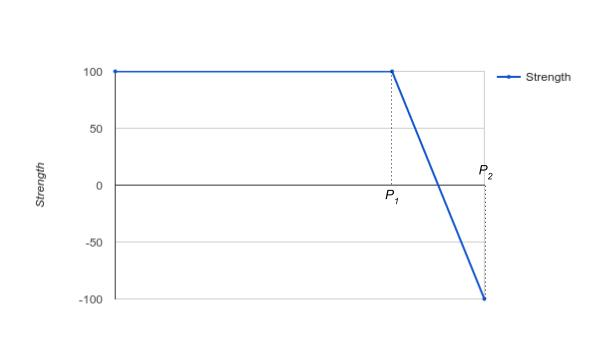
\includegraphics[scale=0.7]{2_value_strength.jpg}
	\caption{ \textit{Graph used to calculate the slope and age strength of a given plant instance where: \textbf{P$_{1}$} represents the value of \textit{start of decline} and \textbf{P$_{2}$} is the \textit{maximum} configured for the given species.} }	
	\label{fig:2_value_strength}
\end{figure}

\begin{figure}
\center
	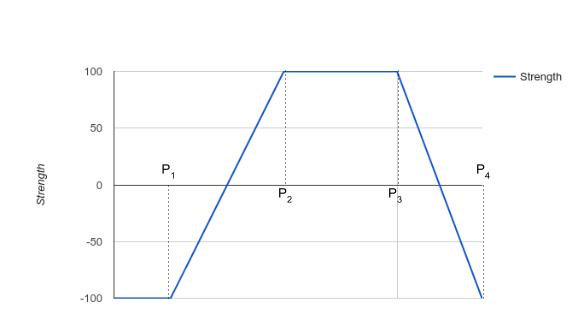
\includegraphics[scale=0.7]{4_value_strength.jpg}
	\caption{ \textit{Graph used to calculate the temperature, illumination and humidity strength of a given plant instance where: \textbf{P$_{1}$} and \textbf{P$_{4}$} are the \textit{minimum} and \textit{maximum} and \textbf{P$_{2}$} and \textbf{P$_{3}$} form the \textit{prime range} configured for the given species.}  }	
	\label{fig:4_value_strength}
\end{figure}

\subsection{Plant Growth}

In the simulation, each plant \textit{P} attempts to grow its roots, its canopy and its height on a monthly basis. Each species has a maximum monthly root growth, canopy growth and height growth which are calculated as outlined in equation \ref{eq:max_growth}. The maximum height, canopy and root size, along with the species age-based start of decline (see section \ref{sec:plant_species}) are used to calculate the amount it must grow each month to reach these maximums by start of decline. Note that this is a simplification as, in reality, plant growth is non-linear as growth slows with increasing size \cite{Paine2012}.

\begin{equation}
MaxGrowth(S) = \frac{Max(S)}{Age_{sod}(S)}
\label{eq:max_growth}
\end{equation}
Where:\textit{MaxGrowth(S)} is the maximum monthly root, canopy or height growth of species \textit{S}; \textit{Max(S)} is the maximum root size, canopy size or height configured for species \textit{S}; \textit{Age$_{sod}$(S)} is the age of start of decline configured for species \textit{S}.\\

The actual root growth, canopy growth and height growth of a plant is directly dependent on its strength (see section \ref{subsec:plant_strength_calc}), however, and is calculated using equation \ref{eq:actual_growth}. This equation only permits growth if the plants strength is positive as it is otherwise deemed too weak to grow and in a state of \textit{survival}. If the strength is positive, the growth is proportional to the plants strength. The maximum growth is therefore only achieved if the plant is at full strength.\\

\begin{equation}
Growth(\textit{P},S) = max(0, Strength(\textit{P}) \times  MaxGrowth(S)
\label{eq:actual_growth}
\end{equation}
Where: \textit{Growth(S)} is the monthly root, canopy or height growth of plant \textit{P} of species \textit{S}; \textit{Strength(P)} is the current strength of \textit{P}; \textit{MaxGrowth(S)} is the maximum monthly root, canopy or height growth calculated for species \textit{S} (see equation \ref{eq:max_growth}).

\subsection{Plant Death}

In order for the simulation to be accurate, it is necessary to model plant death. This can be caused by ageing, the slope being ill-suited or resources being inadequate. On a monthly basis, the probability of death of each plant is calculated based on its strength using equation \ref{eq:probability_of_death} and the plant killed off with the given probability. This equation permits plants to be killed-off only when in a survival state (i.e the strength is negative). If this is the case, the probability of death is proportional to the absolute value of the strength. 

\begin{equation}
Probability_{death}(P) = max(0, \frac{-1 \times Strength(P) + counter}{100})
\label{eq:probability_of_death}
\end{equation}
Where:\textit{Probability{death}(P)} is the probability of death of plant \textit{P};\textit{counter} is a value which increases each month the plants strength is negative, and resets to zero when it becomes positive. This prevents plants from surviving in a survival state for too long.

\subsection{Spawning Plants} \label{subsec:spawning_plants}

In nature, the spawning of new plants ensures species \textit{succession} and \textit{propagation}. In order to accurately model the evolution of an ecosystem it is essential to replicate this spawning mechanism. To do so, seeds are produced annually for each species and are positioned either randomly or at predefined positions. The number of seeds that are produced for a given species is determined by the species configured \textit{annual seed count}. Different seeding mechanisms are used in the simulator depending on the current state of the simulation, as discussed below.\\ 

To ensure species propagation, when plants of the given species are already present in the simulation window, they are used to determine the location for new plant instances. To do so, \textit{n} of these plants are selected at random and seeds placed at random within an annular radius \textit{r} of each. The value of \textit{n} is the \textit{annual seed count} configured for the current specie. The value of \textit{r} is the configured \textit{maximum seeding distance} of the specie. Note that a single plant can be used to spawn multiple seeds if \textit{n} is greater than the number of plants of the given species present in the simulation.\\
This technique is effective in ensuring \textit{propagation} until the number of plant instances present far outweighs the number of seeds, at which point, the \textit{propagation} potential decreases. This is because, as the selection pool for the random seeding plants increases in size, the probability of selecting a seeding plant at a location which will permit propagation decreases. For example, if there are 100 plants of species \textit{s} within a 2 metre square window and 50 are selected for seeding, there is a high probability that a number of them will be selected at the extremities and, therefore, propagate the species further. If there are 10000 plants of the given species, however, the probability of selecting extremity plants and is very low. To overcome this and ensure the initial seeding plants that are selected span a wide area, the simulation window is split into equally sized cells and the seeding plants selected individually from each. \\

If no instance of the given species is present in the simulation (i.e it is the first month) and therefore no seeding plants can be used, the seeds are placed at random within the simulation window.\\ 

A species is deemed shade-loving if its configured minimum daily illumination is zero. Such species thrive in the undergrowth of other plants. Spawning shade-loving species in the same way as other plants would drastically limit their chance of survival because the probability of a random seed location falling in the canopy of an existing plant is very low. For this reason, when there are no instances of the given shade-loving species present in the simulation window, the seed locations are located at random under the canopy of existing plants. If instances of the plant species are already present, however, they are used to propagate the seeds, just like with other, non shade-loving, plant species.

\subsection{Performance} \label{subsec:ecosytem_performance}

The number of plants present in the simulation will heavily influence its performance as the strength of each plant needs to be recalculated on a monthly basis. To test the influence of plant count on simulation execution time, a simulation is run with a single species of plant and the monthly processing time analysed alongside the number of plants present. The plant used is grass as is has no canopy and very minimal root coverage, therefore permitting a large number of instances to grow simultaneously (see appendix \ref{AppendixB} for properties of the specie). The resources were set to be optimal for maximizing plant count and minimizing intra-plant competition. The simulation is started with only a single instance and, as the simulation progresses and seeding is performed, the number of instances increases. The results are summarized in Figure \ref{fig:ecosimulator_test_plant_count} and show that the processing time increases linearly with plant count. The jump at the 65 thousand plant mark occurred repeatedly over multiple tests. Although just a hypothesise, the most likely cause is that it is a tipping point at which page swapping starts to occur due to saturated RAM.\\

\begin{figure}
\center
	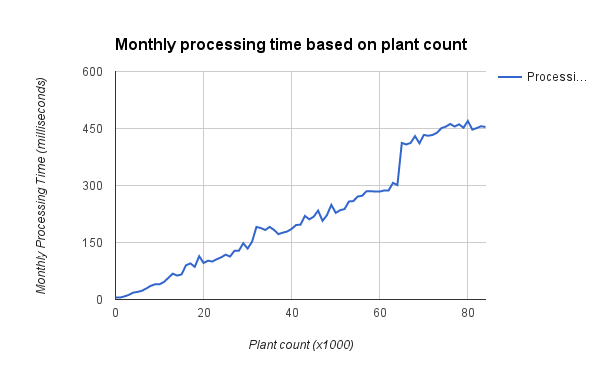
\includegraphics[scale=0.7]{ecosimulator_test_plant_count.png}
	\caption{ \textit{Processing time based on plant count. Total simulation time for 100 years: 271 seconds}}	
	\label{fig:ecosimulator_test_plant_count}
\end{figure}

Another property that heavily impacts performance is the root and canopy growth. As roots and canopies grow, they will cover more grid cells of the simulation window, and more calculations will be required per individual cell. To analyse the impact of plant growth, a base species \textit{S$_{base}$} is created with a given root and canopy growth rate. Then, two species \textit{S$_{X2}$} and \textit{S$_{X3}$} are created with identical properties to \textit{S$_{base}$} but with twice and thrice the growth rates, respectively (see appendix \ref{AppendixB} for species details). Separate simulations are run with each species but with identical available resources and, on a monthly basis, the number of plants present in the simulation, along with the monthly processing time, are analysed. Given this information, it is possible to track the average monthly execution time per plant throughout the simulation. It is important to normalise this based on the number of plants as faster growing plants will naturally reduce the total plant count for the simple reason that they will require and be able to access resources from a larger number of grid cells. As can be seen in the results plotted in figure \ref{fig:ecosimulator_test_per_plant}, the processing times are similar to begin with and then increase proportionally to the species growth rate. For the fastest growing plant specie, \textit{S$_{X3}$}, it took 166 seconds to simulate one hundred years.

\begin{figure}
\center
	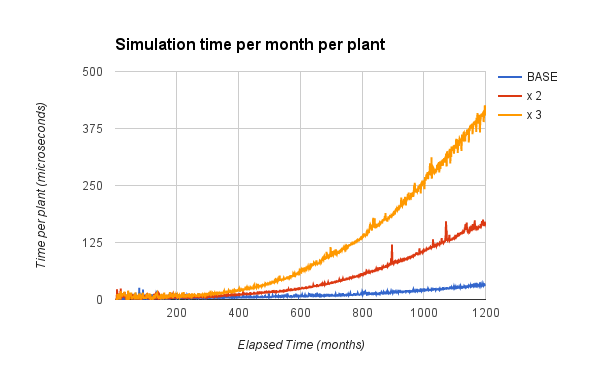
\includegraphics[scale=0.7]{ecosimulator_test_per_plant.png}
	\caption{ \textit{Evolution of the monthly processing time normalised based on plant count. The processing time increases as the plants grow larger since they cover more grid cells. Total simulation time for one hundred years: ~49 seconds for \textit{S$_{base}$}, ~122 seconds for \textit{S$_{X2}$} and 166 seconds for \textit{S$_{X3}$}}}
	\label{fig:ecosimulator_test_per_plant}
\end{figure}

\subsection{Results} \label{subsec:ecosystem_simulator_results}

To test the resulting spatial distribution of plant communities in their work, Lane and Przemyslaw \cite{Lane2002} attempt to reproduce three important properties of nature: \textit{Self-thinning}, \textit{succession} and \textit{propagation}. To test the ecosystem simulator, we employ the same methodology as Lane and and Przemyslaw \cite{Lane2002} and attempt to reproduce these core properties of nature. Other tests are also performed to ensure plant instances thrive better in environments suited to their individual resource requirements.\\

\textbf{SELF-THINNING TEST}\\

As plants grow, their resource requirements increase and, as a direct consequence, inter-plant competition for resources increases. Eventually, the competition becomes too intense and resources too scarce, leading to more vigorous plants starving smaller plants. At this point, \textit{self-thinning} begins and plant densities decrease \cite{Lane2002}.\\
To test whether self-thinning is successfully modelled in the ecosystem simulator, three simulations are run differing only in the configured soil moisture and the plant count tracked throughout. As described previously, self-thinning occurs because of insufficient resources. By modifying only available humidity in each simulation, its affect on self-thinning becomes apparent. As can be seen in the results summarized in figure \ref{fig:self_thinning_test_results}, the plant count increases at first, reaches a maximum and decreases thereafter. This is the expected behaviour of self-thinning. Furthermore, it is apparent that the maximum plant count increases with the humidity available, therefore showing that the tipping point depends on available resources.\\

\begin{figure}
\center
	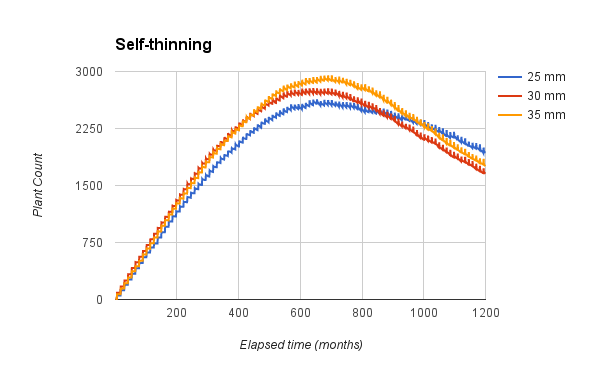
\includegraphics[scale=0.7]{self_thinning.png}
	\caption{ \textit{Self thinning test: plant count tracked throughout three separate simulations differing only in available humidity. For all three runs the plant density reaches a maximum tipping-point after which plant density reduces. Note that the more available moisture there is, the more severe the slope of descent is following the tipping point. This is because, with more soil moisture available, plants thrive and reach greater sizes. Because of this increased spatial coverage, the killing off of smaller plants is more severe. So, although the plant count is smaller by the end of the simulations when there is more humidity, the average plant size is larger.}}
	\label{fig:self_thinning_test_results}
\end{figure}

\textbf{SUCCESSION TEST}\\

Given plant species \textit{A} with a fast growth rate and species \textit{B} with a slower growth rate but higher shade tolerance. At first, the faster growing species A will dominate and flourish but, with time, the slower growing, but more shade-tolerant species B will flourish and dominate. This is the \textit{succession} property. To test \textit{succession} in the ecosystem simulator, two plant species \textit{S$_{fast}$} and \textit{S$_{slow}$} are created differing only in their growth rate and illumination properties (see appendix \ref{AppendixB} for details) and a simulation run with these two species under optimal conditions. During the simulation, the appearance and average size of the two plant species are monitored to determine the dominating specie. The results are analysed and illustrated in figure \ref{fig:succession_plants_avg_size}. A snapshot of the simulation window is taken at ten year intervals and displayed in figure \ref{fig:succession_plants_render}. Both these figures show that \textit{S$_{fast}$} dominates at first (~300 months in) followed by \textit{S$_{slow}$} (~500 months in). A balance is found thereafter.\\

\begin{figure}
\center
	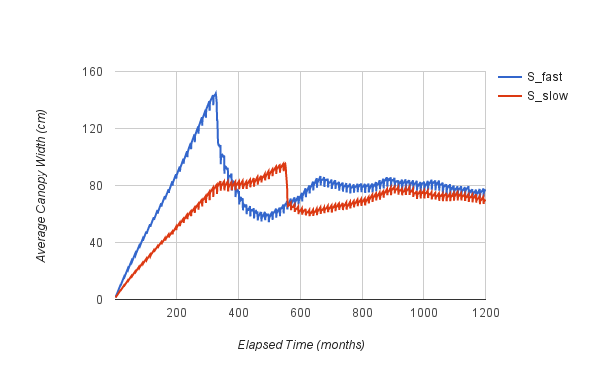
\includegraphics[scale=0.7]{succession_plant_avg_size.png}
	\caption{ \textit{Succession Test: Average size of the slow growing S$_{slow}$ (red) and fast growing S$_{fast}$ (blue) throughout a simulation run in optimal conditions. Note that the plant count drops severely at the 300 and 500 mark for S$_{fast}$ and S$_{slow}$ respectively as resources are configured such that conditions are ideal for these species. This leads to a large quantity of them dying of age and, because the difference between start of decline and maximum age configured for these species is very small, it is done performed very sharply.}}
	\label{fig:succession_plants_avg_size}
\end{figure}

\begin{figure}
\center
	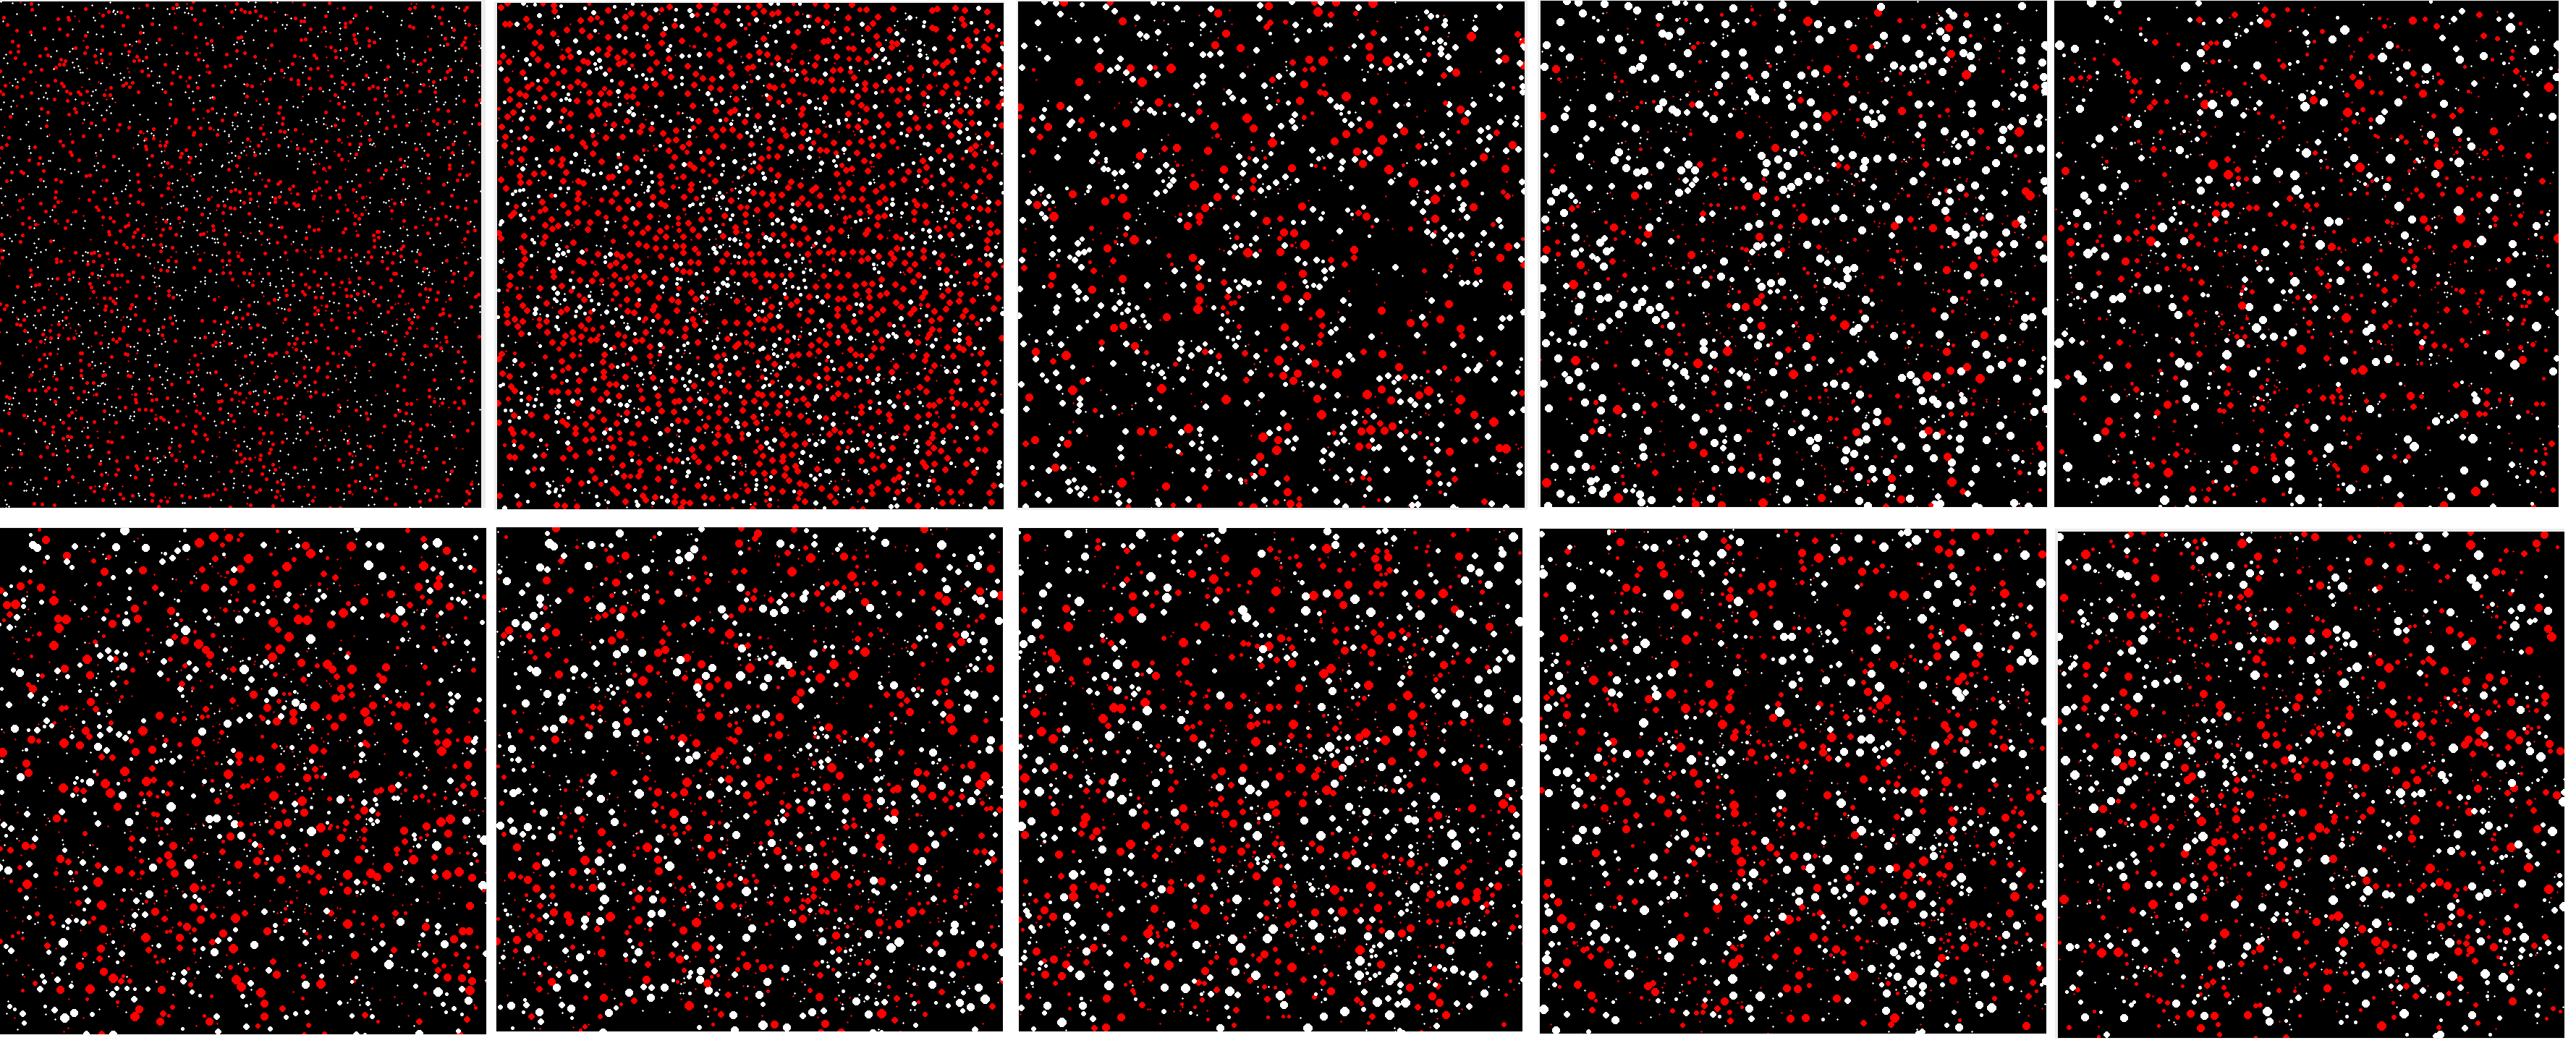
\includegraphics[width=\textwidth]{succession_plants_render.png}
	\caption{ \textit{Succession Test: Appearance of the slow growing S$_{slow}$ (white) and fast growing S$_{fast}$ (red) at different times during the simulation. From left-to-right, top-top-bottom: 10, 20, 30, 40, 50, 60, 70, 80, 90 and 100 years.}}
	\label{fig:succession_plants_render}
\end{figure}

\textbf{PROPAGATION TEST}\\

The \textit{propagation} property simply states that plants \textit{propagate} in clusters surrounding the seed plants. To ensure propagation is modelled, a simulation is run with a single starting grass seed (see appendix \ref{AppendixB} for species details) and its evolution tracked throughout. Figure \ref{fig:propagation_test_render} shows that iterative propagation through annual seeding enables a single seed plant to colonize the entirety of the terrain. Note that, although it does show propagation is reproduced, it is unrealistically slow. This is caused by the seeding algorithm used. As discussed in section \ref{subsec:spawning_plants}, in order to promote propagation, the simulation window is split into grids and seeding plants selected separately from each cell. Although this increases the spatial coverage of the seeding plants, it still fails to propagate effectively when the number of grid cells in which the given species appears is large as the probability of selecting a grid cell from the edge (which would lead to seeding) decreases with the grid coverage of the given specie. A worthwhile extension to this work would be to implement the ability to locate border grid cells and use them more extensively during seeding. This could be done by, for example, sorting the grid cells in order of the species count they contain as border cells would naturally be less dense. \\

\begin{figure}
\center
	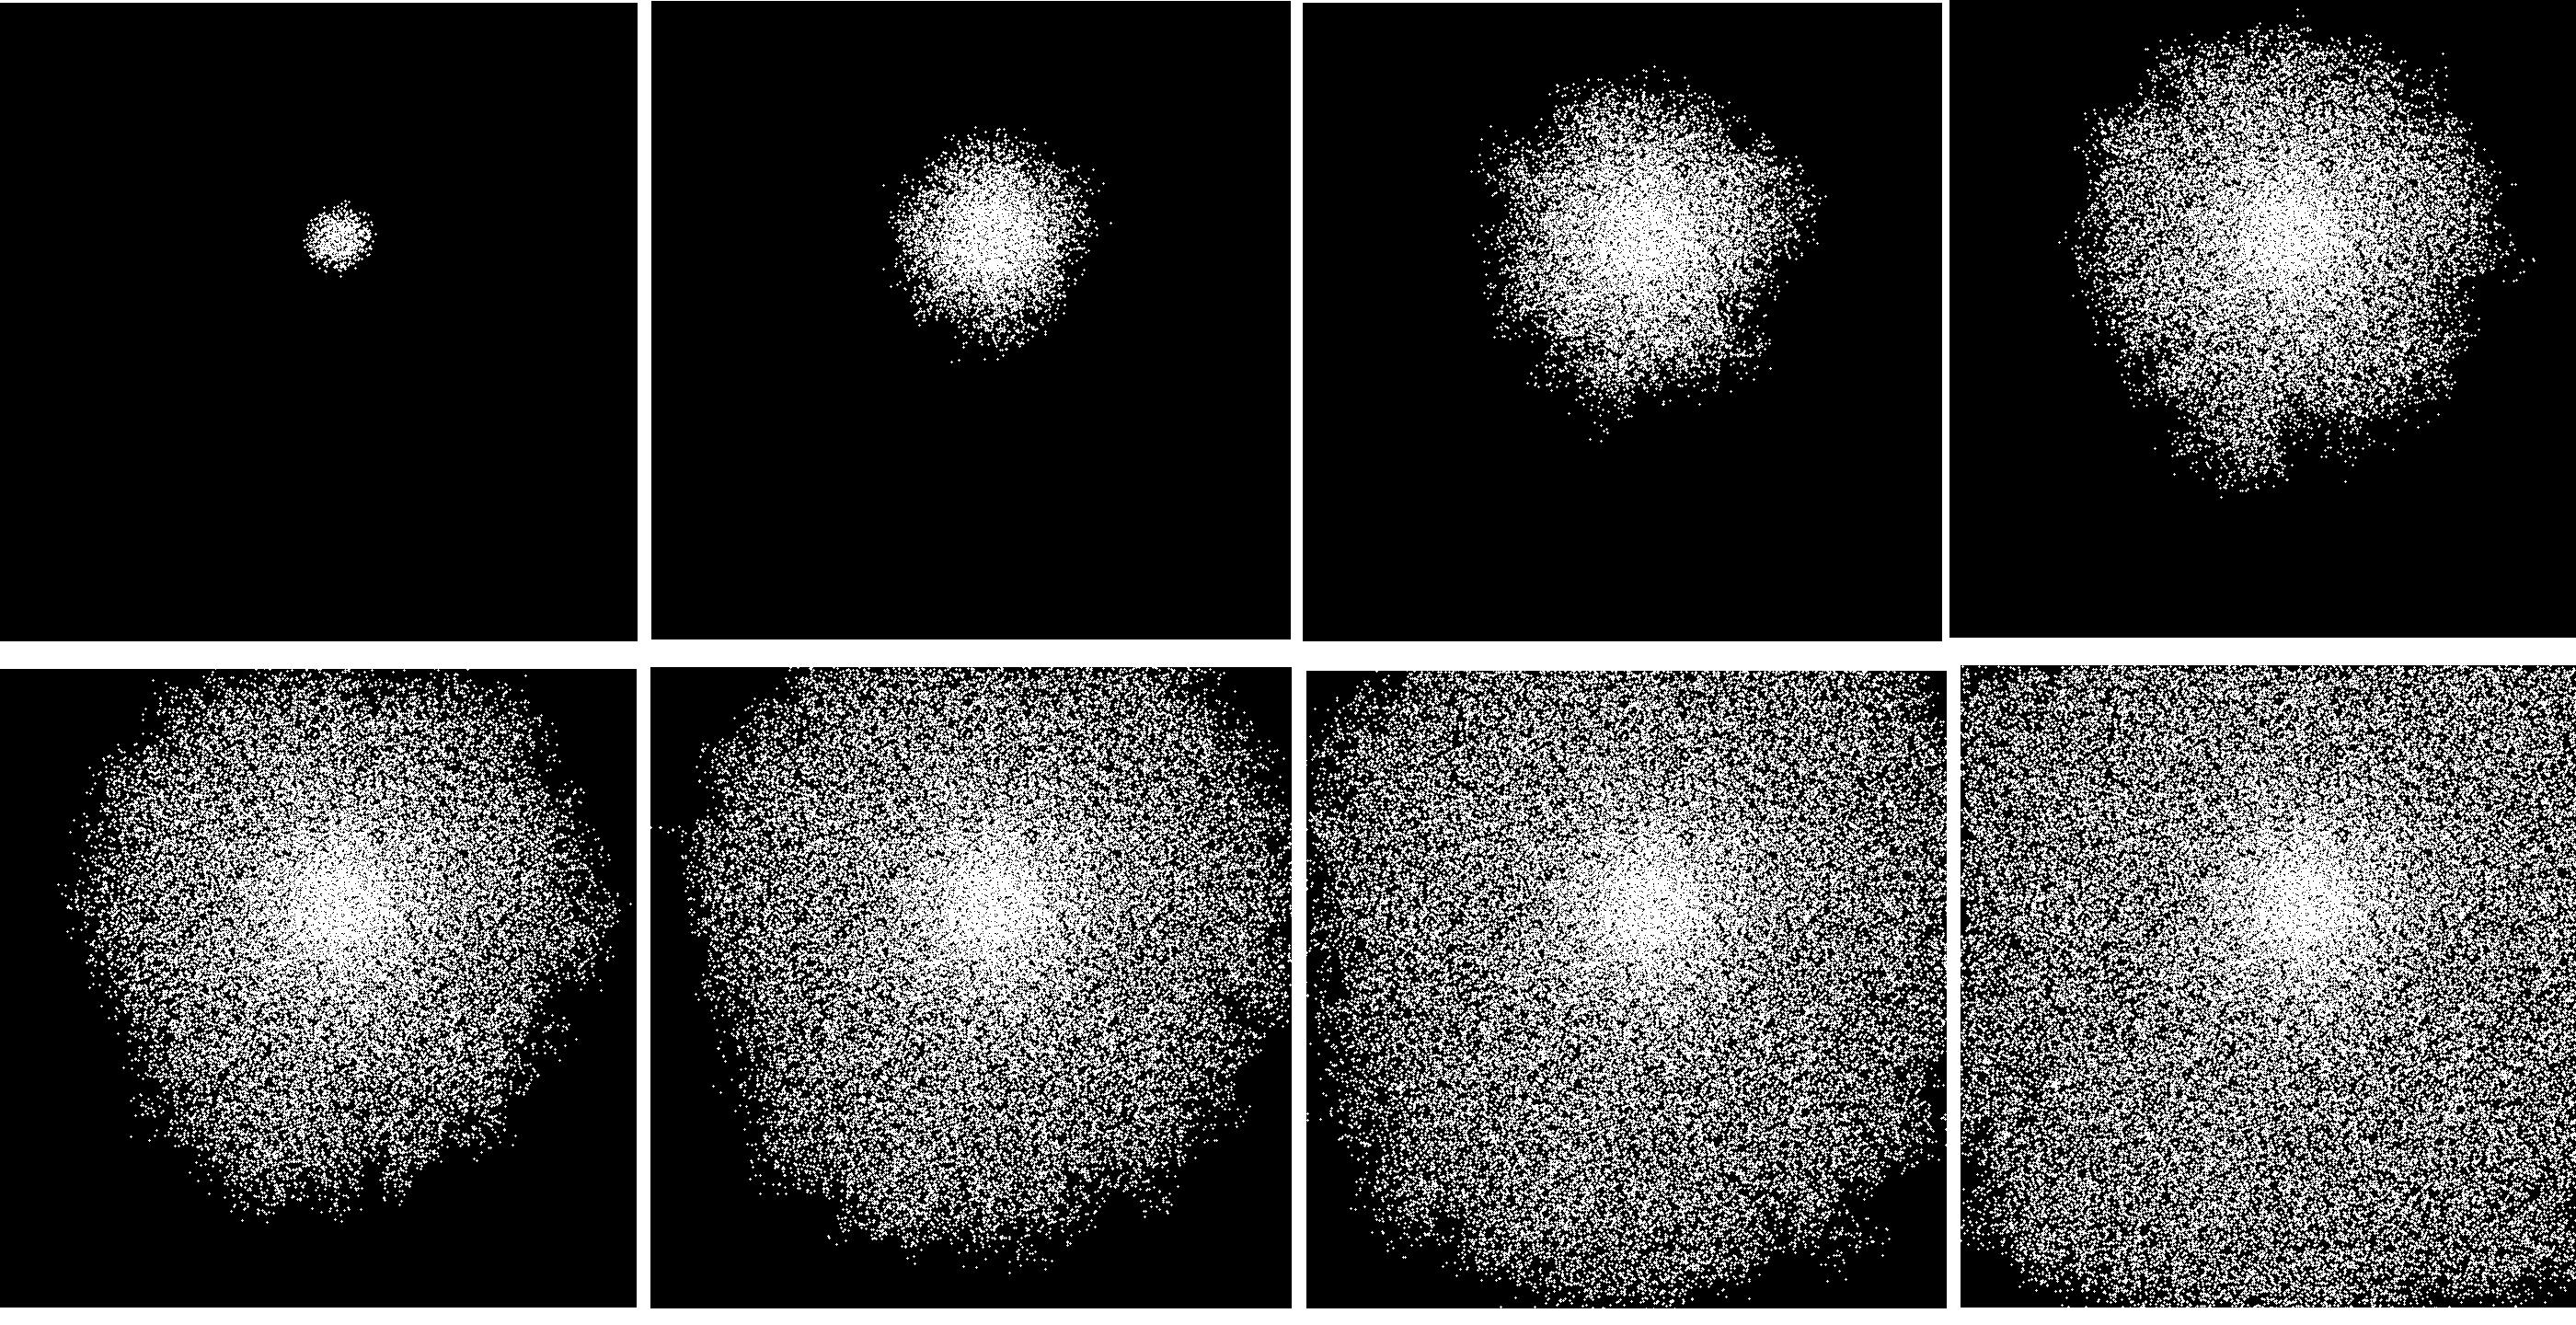
\includegraphics[width=\textwidth]{propagation_test_render.png}
	\caption{ \textit{Propagation Test: Evolution through time of a simulation starting from a single seed plant of grass. From left-to-right, top-to-bottom: 2, 10, 20, 30, 40, 50, 60, 70 years in.}}
	\label{fig:propagation_test_render}
\end{figure}

\textbf{VARYING RESOURCE TEST} \\

To ensure a given plant species thrives better when the environment is more suitable, multiple simulations are run with a single species \textit{S$_{base}$} (see appendix \ref{AppendixB} for species properties) varying only in available humidity. Throughout the simulation, the average plant canopy width is tracked to monitor the strength of the plants. As can be seen by the results plotted in figure \ref{fig:varying_resource_test}, plants thrive better in environments better suited to their resource requirements.\\

\begin{figure}
\center
	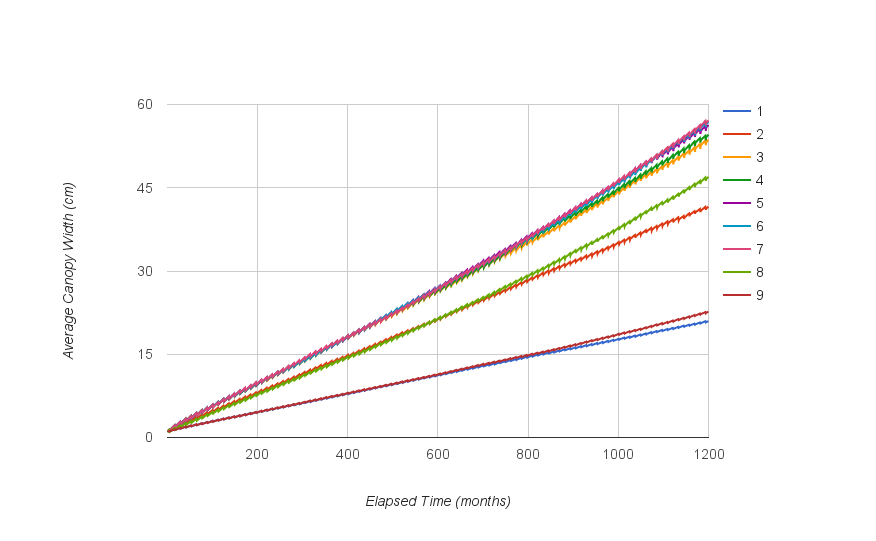
\includegraphics[width=\textwidth]{varying_resource_test.png}
	\caption{ \textit{Varying resource test: Average canopy width throughout simulations varying only in available moisture and with only plant species \textit{S$_{base}$}. It shows that the average canopy width is low when the configured humidity is outside the species optimal humidity range (22mm and 38mm), improves as it approaches optimal range (24mm and 36mm) and reaches its peak when the humidity is within the optimal range (26mmn, 28mm, 30mm, 32mm and 34mm).}}
	\label{fig:varying_resource_test}
\end{figure}

\textbf{SHADE TEST}\\

Plants that are heavily dependent on illumination struggle to grow in areas shaded by the canopy of larger plants. To ensure this is modelled in the ecosystem simulator, a simulation is run with two species: \textit{S$_{smallroots}$} and grass (see appendix \ref{AppendixB} for species details). \textit{S$_{smallroots}$} is a custom species created for the purpose of this test which has a very small root growth value. This is important so as to focus on the effects of illumination and minimize the influence of drought. Figure \ref{fig:shade_test}, which illustrates the state of the simulation after ten years, shows the grass struggling to grow in areas directly below the canopies of \textit{S$_{smallroots}$}.\\

\begin{figure}
\center
	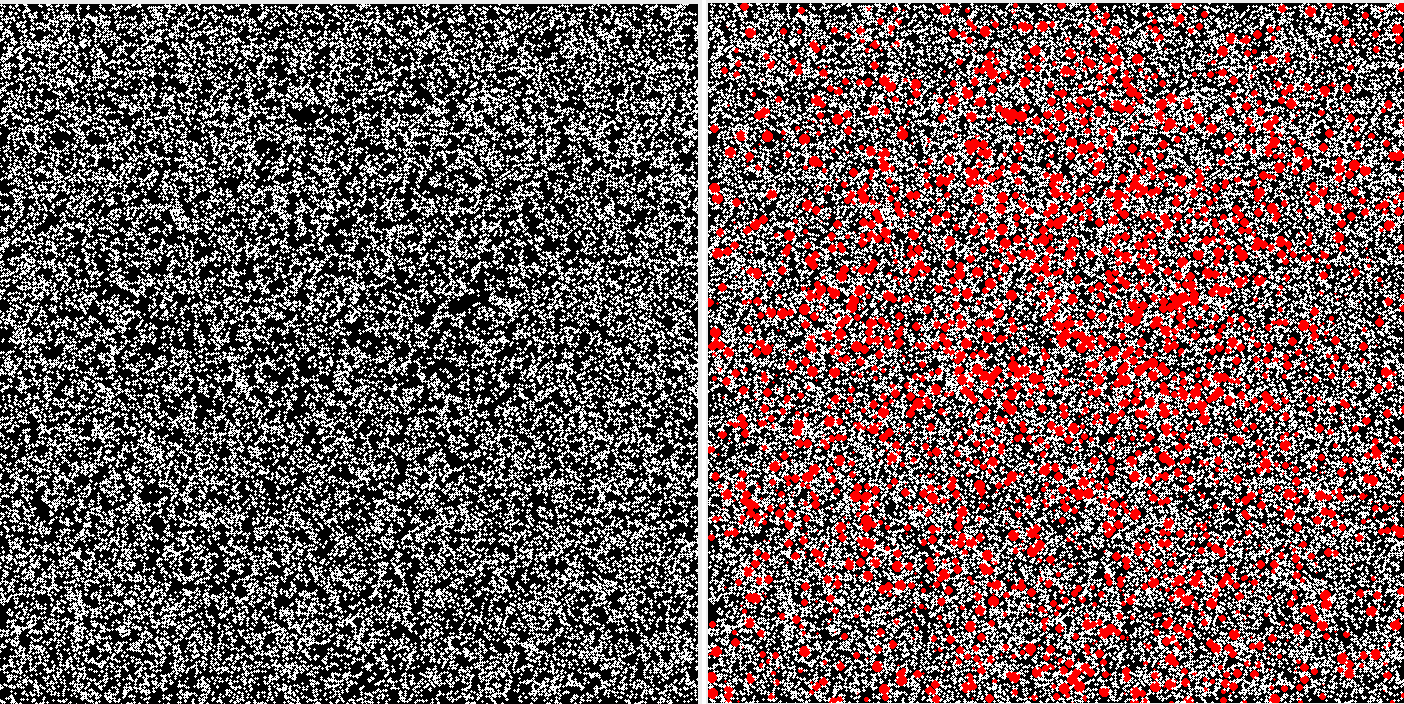
\includegraphics[width=\textwidth]{shade_propagation_test.png}
	\caption{ \textit{Shade Test: Results of a simulation run with \textit{S$_{smallroots}$} (red), grass (white) after 10 years. Top-left: Rendered with both species. Top-right: Only grass rendered in order to clearly visualise the empty areas at the exact locations the canopies of \textit{S$_{smallroots}$} appear. Bottom: The same simulation run with only grass, clearly showing the empty areas disappear.}} 
	\label{fig:shade_test}
\end{figure}

\textbf{SHADE-LOVING TEST}\\

As discussed in \ref{subsec:spawning_plants}, species which strive in shaded areas are deemed shade-loving. The shade can be caused by the terrain relief or by the shadow cast by the canopy of taller plants. To test whether the ecosystem simulator successfully caters for such plant species, a simulation identical to the shade test is run but with shade-loving species \textit{S$_{shadeloving}$} added (see appendix \ref{AppendixB} for species details). As seen by the snapshot of the simulation after fifteen years illustrated in figure \ref{fig:shade_loving_test}, instances of \textit{S$_{shadeloving}$} only appear in areas covered by the canopies of \textit{S$_{smallroots}$}.

\begin{figure}
\center
	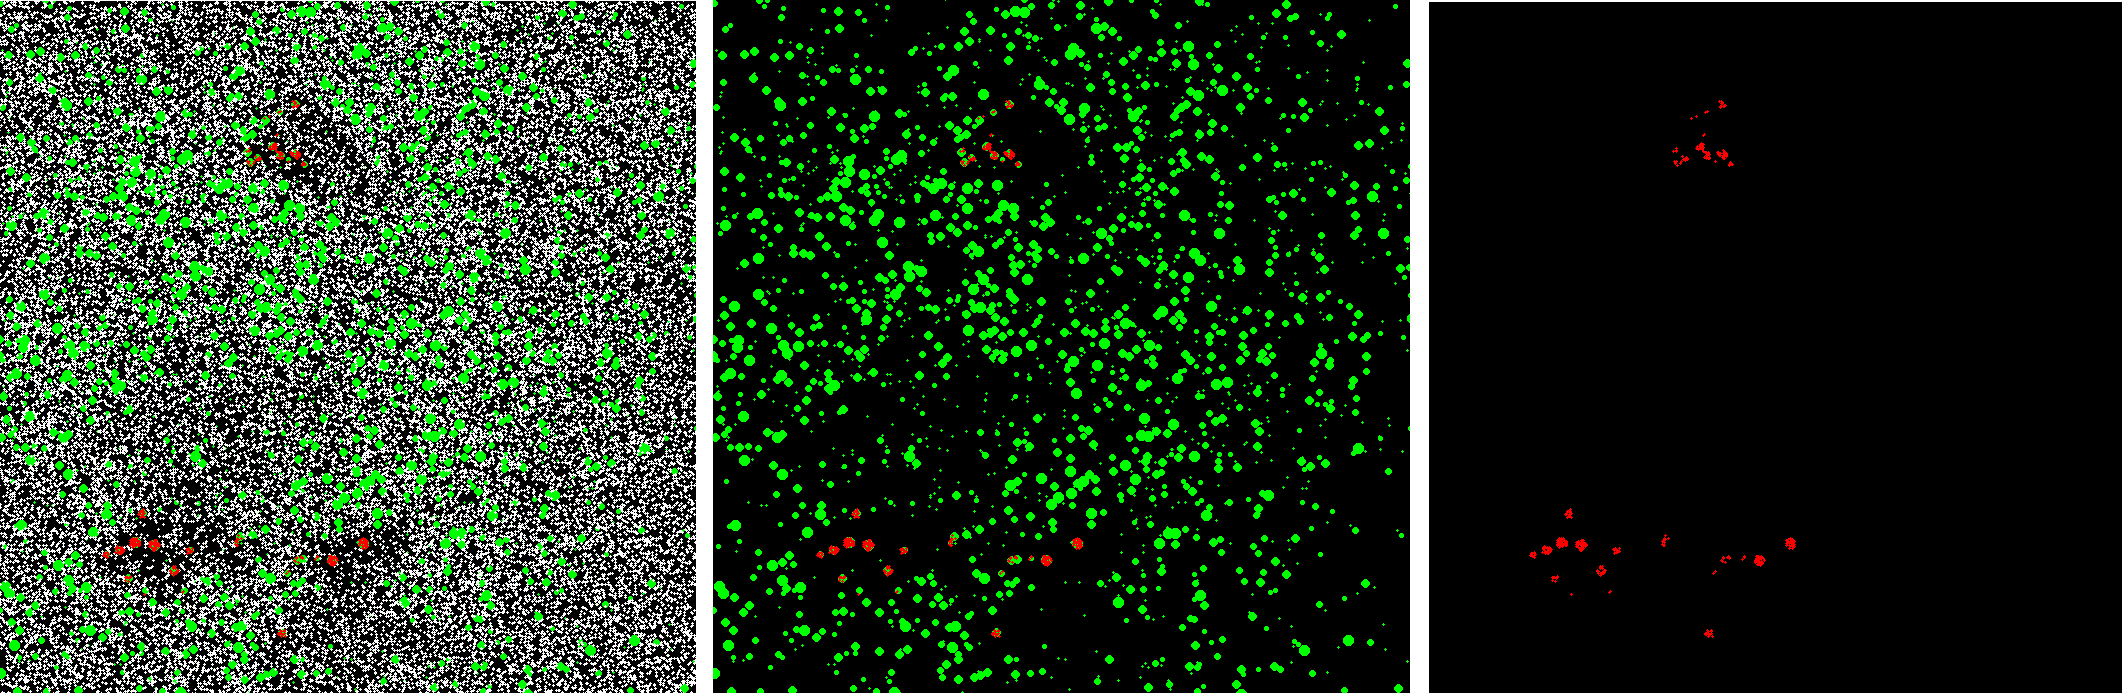
\includegraphics[width=\textwidth]{shade_loving_test.png}
	\caption{ \textit{Shade Loving Test: Simulation with \textit{S$_{smallroots}$} (red), grass (white) and \textit{S$_{shadeloving}$} (green) after 15 years. Left: All species rendered. Right: All except \textit{S$_{smallroots}$} rendered. It shows clearly that the only instances of \textit{S$_{shadeloving}$} which survive are those under the canopies of \textit{S$_{smallroots}$} (red).}}
	\label{fig:shade_loving_test}
\end{figure}
